\section{Marco teórico}

\subsection{Punto estático de operación}

El punto estático de operación es el punto donde está trabajando u operando el transistor. Se encuentra
conformado por la corriente del colector (ICQ) y la tensión colector-emisor (VCEQ). El punto se encuentra dentro de una recta la
cual se obtiene mediante IC y VCE. A continuación se muestra una aproximación de las curvas de transferencia de un transistor
BJT

\subsection{Amplificador de potencia}
Un amplificador de potencia es un dispositivo electrónico que toma una señal de entrada de baja potencia y la amplifica
para producir una señal de salida de mayor potencia. Los amplificadores de potencia se clasifican por su configuración de circuito,
como amplificadores de clase A, B, AB y C. Cada clase tiene su propio conjunto de características y beneficios.

\subsubsection{Amplificador de potencia de clase A}

El amplificador de Clase A es la forma más simple de amplificador de potencia que
utiliza un solo transistor de conmutación en la configuración de circuito de emisor común
estándar como se ha visto anteriormente para producir una salida invertida. El transistor
siempre está polarizado en .ON”para que conduzca durante un ciclo completo de la forma
de onda de la señal de entrada, produciendo la mínima distorsión y la máxima amplitud de
la señal de salida.

Esto significa que la configuración del amplificador de clase A es el modo de funcionamiento ideal, ya que no puede haber distorsión de cruce o desconexión a la forma de onda
de salida incluso durante la mitad negativa del ciclo. Las etapas de salida del amplificador
de potencia de Clase A pueden usar un único transistor de potencia o pares de transistores
conectados entre í para compartir la corriente de alta carga. Una de las principales desventajas de los amplificadores de potencia y especialmente del amplificador de Clase A es
que su eficiencia de conversión general es muy baja, ya que las grandes corrientes significan
que se pierde una cantidad considerable de energía en forma de calor.

\subsubsection{Amplificador de potencia de clase B}

Los amplificadores de Clase B usan dos o más transistores polarizados de tal forma que
cada transistor solo conduce durante un medio ciclo (realmente, ¸casi”medio ciclo) de la
onda de entrada. Tienen un rendimiento muy superior a los de Clase A y su diseño no es
muy complicado, pero sus aplicaciones se limitan enormemente debido a una característica
su propio diseño: una distorsión llamada de ¸cruce por cero”. Aún así, se utilizan incluso
en amplificadores que no requieran buena fidelidad y sí facilidad de diseño y rendimiento,
como los amplificadores de bocinas y megáfonos de mano.


\subsubsection{Amplificador de potencia de clase AB}

El dispositivo se polariza en la zona lineal pero en un punto muy próximo al extremo
de respuesta lineal. Esta configuración es una variante de la etapa de tipo B en la que
se sacrifica la disipación de una pequeña cantidad de potencia cuando opera sin señal, a
cambio de evitar la zona muerta de respuesta,amplificador clase AB opera como un clase
A. Mientras que, a altos niveles de salida, la señal sobrepasa el punto cero de cruce y se
comienza a comportar como un clase B.

\subsubsection{Amplificador de potencia de clase C}

Los amplificadores de potencia en clase C parten de la premisa siguiente: no se trata
de amplificar con calidad la señal de entrada, se trata simplemente de amplificar la señal
de entrada de modo que a la salida se obtenga el máximo rendimiento posible pero sólo
para un rango de frecuencias muy reducido, en torno a una de resonancia”.En torno a la
frecuencia de resonancia, estos amplificadores obtienen una ganancia altísima; fuera de esta
frecuencia, la amplificación es muy reducida y el consumo es mínimo.

\subsection{Amplificador diferencial}

El amplificador diferencial es la etapa de entrada característica de un amplificador operacional. No tiene capacitores de acoplamiento ni de paso, lo que implica que esta directamente
acoplado. Por esto, puede amplificar cualquier frecuencia incluyendo la señal de DC, que es
equivalente a una señal de frecuencia cero. La corriente de cola en un amplificador diferencial se divide exactamente entre los transistores cuando estos son idénticos.Cuando los dos
transistores de un amplificador diferencial no son idénticos, las dos corrientes de base son
diferentes. La corriente de desajuste de la entrada se define como la diferencia entre las dos
corrientes de base. La corriente de polarización de la entrada se define como el promedio de
las dos corrientes de base.

\subsection{Respuesta en frecuencia}

La respuesta en frecuencia de un amplificador operacional en lazo cerrado o lazo abierto
se defiene como el límite de alta frecuencia y el límite de baja frecuencia. En estos límites, la
ganancia de voltaje se reduce un 0.707 del valor máximo de voltaje, en el rango de frecuencia
útil.
El ancho de banda para pequeña señal es la diferencia entre el límite de alta frecuencia
y el límite de baja frecuencia.

La respuesta en frecuencia de un amplificador se puede representar gráficamente mediante un diagrama de Bode.

\begin{figure}[ht]
    \centering
    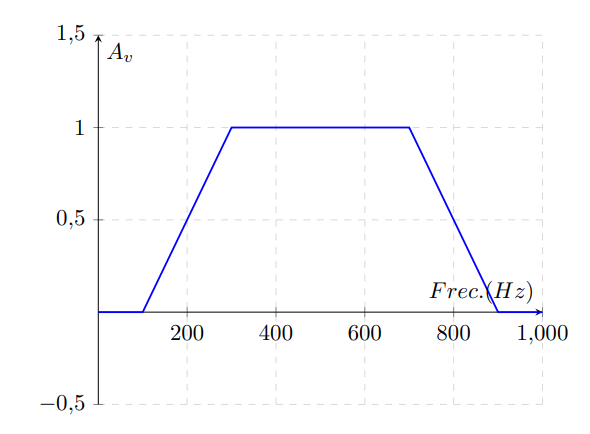
\includegraphics[width=0.5\textwidth]{src/images/marco-teorico/diagrama-de-bode.png}
    \caption{Diagrama de Bode}
    \label{fig:mt-diagrama-de-bode}
\end{figure}

Además se debe agregar que:

\begin{itemize}
    \item Para frecuencias medias, los capacitores de acople y desacople se comportan como un
cable, es decir, un cortocircuito.
    \item Para frecuencias altas, las limitaciones en frecuencia de los dispositivos activos condicionan la frecuencia máxima de operación del amplificador
    \item Para frecuencias bajas, el efecto de los condensadores de acoplo y desacoplo es importante
\end{itemize}

\subsection{Realimentación en un amplificador}

La realimentación consiste en combinar una muestra de la señal de salida del amplificador
con la señal de entrada, de modo tal que se modifican las características generales del
sistema. Puede ser positiva o negativa.


\begin{figure}[ht]
    \centering
    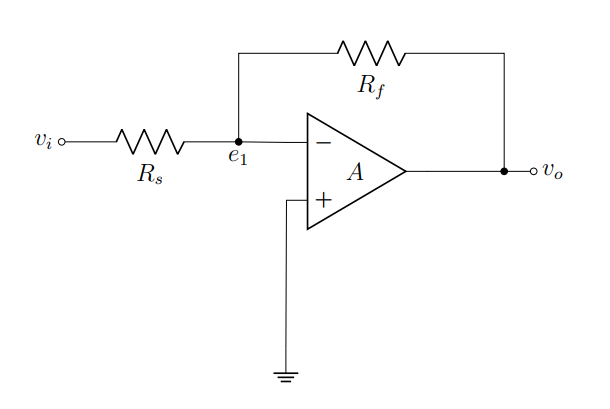
\includegraphics[width=0.5\textwidth]{src/images/marco-teorico/amplificador-inversor.png}
    \caption{Amplificador inversor}
    \label{fig:mt-amplificador-inversor}
\end{figure}


\subsubsection{Realimentación negativa}

La realimentación es negativa cuando el valor de la señal de salida es menor que sin la
realimentación. Para ello, la señal de salida que se toma como muestra es aplicada opuesta
en fase a la señal de entrada.
La realimentación negativa disminuye la ganancia del amplificador y a pesar de ello, la
inmensa mayoría de los amplificadores utilizan esta variante de realimentación debido a las
muchas ventajas que se obtienen con la aplicación de este principio, tales como el aumento
de la estabilidad y el ancho de banda, la disminución de las distorsiones de frecuencia y de
no linealidad así como del ruido y el cambio en las resistencias de entrada y salida. Todo
esto incrementa notablemente la calidad y versatilidad de los amplificadores.
Los cambios provocados por el envejecimiento de los componentes y dispositivos, su
reemplazo u otras causas, las variaciones de temperatura, etcétera, se reflejan en las alteraciones que puede sufrir la ganancia de un amplificador con relación a su valor original. Tales
alteraciones son de hecho reducidas con la realimentación negativa, a tal extremo que su ganancia puede llegar a depender solamente de las características de la red de realimentación,
cuando la ganancia de lazo es mucho mayor que la unidad.

\subsubsection{Realimentación positiva}

La realimentación es positiva cuando el valor de la señal de salida es mayor que sin
la realimentación. Esto se logra cuando la señal de salida que se toma como muestra es
aplicada en fase con la señal de entrada.
El resultado de la realimentación positiva es contrario a la realimentación negativa, es
decir se incrementa el ruido, la ganancia y la distorsión, disminuyendo el ancho de banda y
la estabilidad, por lo cual este efecto no es aconsejable para los amplificadores, sin embargo,
puede ser aprovechado con gran eficacia en los circuitos osciladores
